%%%%%%%%%%%%%%%%%%%%%%%%%%%%%%%%%%%%%%%%%%%%%%%%%%%%%%%%%%%
% --------------------------------------------------------
% Tau
% LaTeX Template
% Version 2.4.4 (28/02/2025)
%
% Author: 
% Guillermo Jimenez (memo.notess1@gmail.com)
% 
% License:
% Creative Commons CC BY 4.0
% --------------------------------------------------------
%%%%%%%%%%%%%%%%%%%%%%%%%%%%%%%%%%%%%%%%%%%%%%%%%%%%%%%%%%%

\documentclass[9pt,a4paper,column,twoside]{tau-class/tau}
\usepackage[english]{babel}

%% Spanish babel recomendation
% \usepackage[spanish,es-nodecimaldot,es-noindentfirst]{babel} 

%% Draft watermark
% \usepackage{draftwatermark}

%----------------------------------------------------------
% TITLE
%----------------------------------------------------------

\journalname{Intro Microelectronic Circuits with Laboratory}
\title{The MOS Differential Pair}

%----------------------------------------------------------
% AUTHORS, AFFILIATIONS AND PROFESSOR
%----------------------------------------------------------

\author[1]{Henry Tejada Deras}
\author[1]{Anika Mahesh}
\author[1]{Elias Tuthill}

%----------------------------------------------------------

\affil[1]{Franklin W. Olin College of Engineering}

%----------------------------------------------------------
% FOOTER INFORMATION
%----------------------------------------------------------

\institution{Franklin W. Olin College of Engineering}
\footinfo{Intro Microelectronic Circuits with Laboratory}
\theday{TBD}
\leadauthor{Tejada Deras et. al.}

%----------------------------------------------------------

\begin{document}
		
    \maketitle 
    \thispagestyle{firststyle} 
    % \tauabstract 
    % \tableofcontents
    % \linenumbers 
    
%----------------------------------------------------------

\section{Differential Pair Current–Voltage Characteristics}
	\subsection{Results}
    \begin{figure}[H]
		\centering
		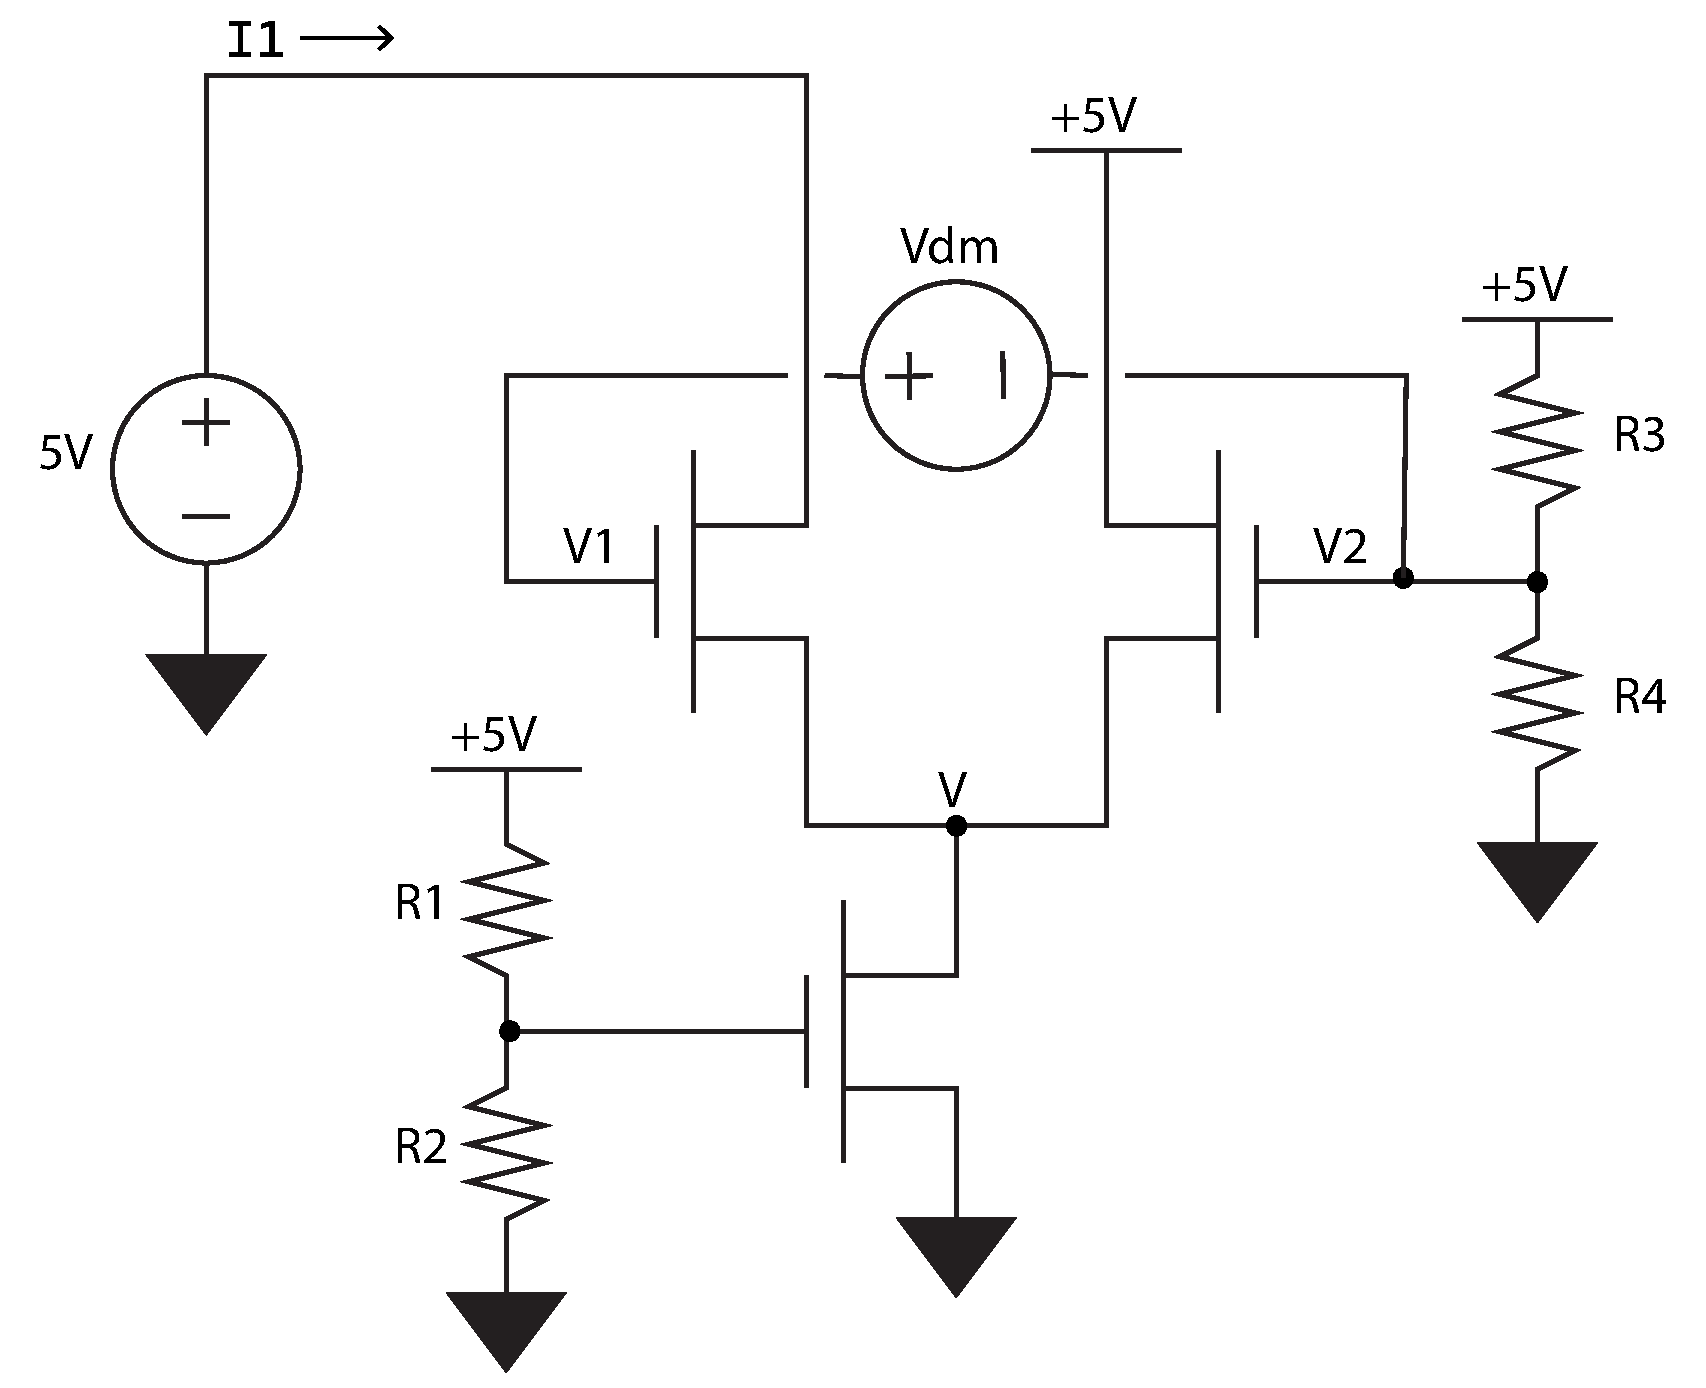
\includegraphics[width=0.6\linewidth]{../diagrams/lab5-diagram1.pdf}
	\caption{Experimental setup for the first part of Experiment 1.}\label{fig:cd1}
	\end{figure}

    \begin{figure}[H]
		\centering
		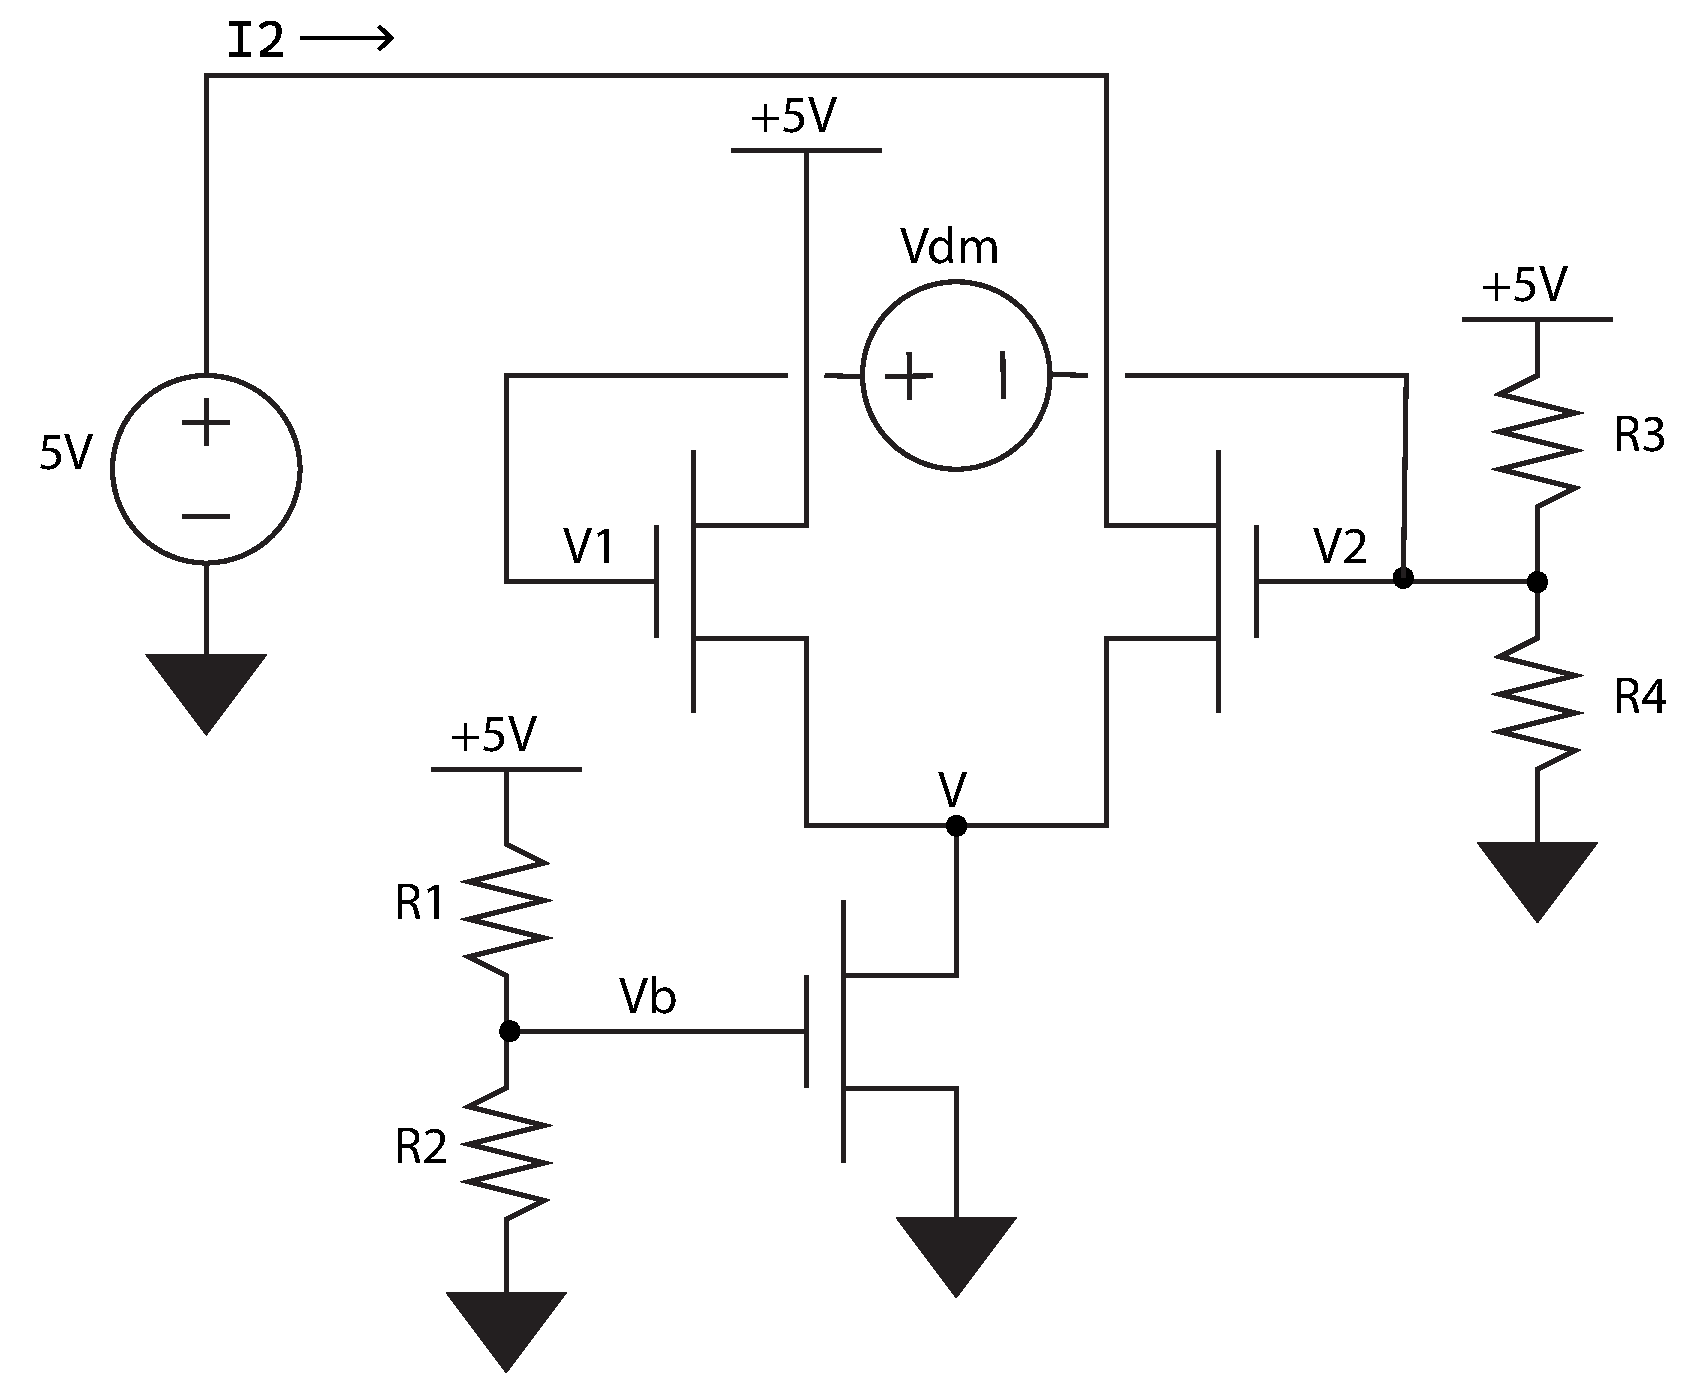
\includegraphics[width=0.6\linewidth]{../diagrams/lab5_diagram2.pdf}
	\caption{Experimental setup for the second part of Experiment 1.}\label{fig:cd2}
	\end{figure}

    \begin{figure}[H]
		\centering
		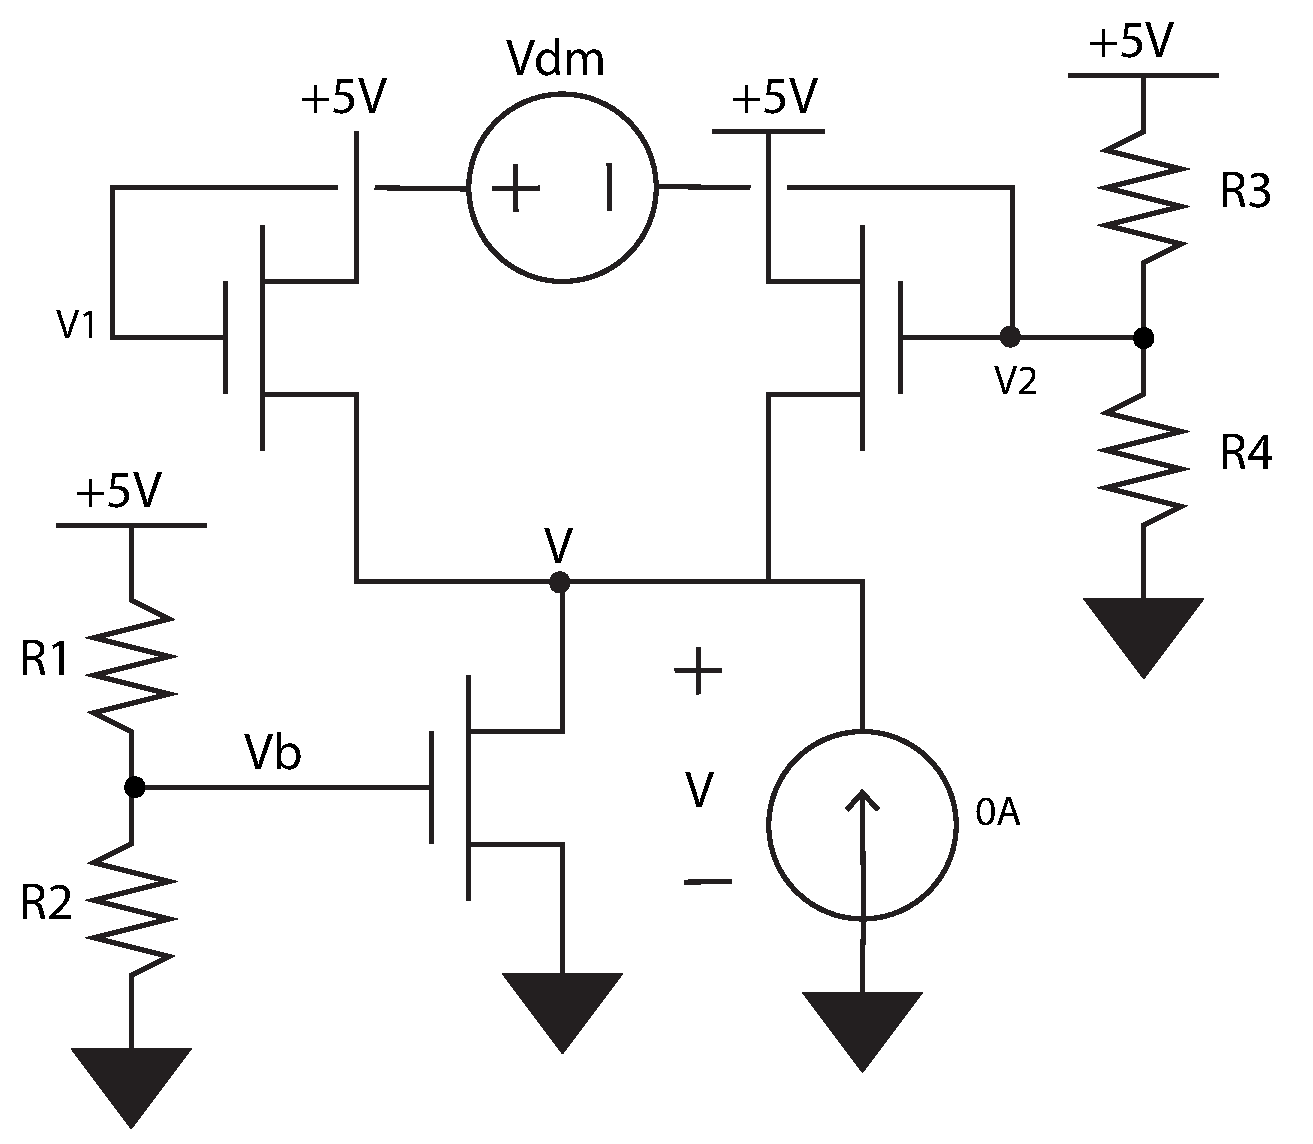
\includegraphics[width=0.6\linewidth]{../diagrams/lab5-diagram3.pdf}
	\caption{Experimental setup for the third part of Experiment 1.}\label{fig:cd3}
	\end{figure}
	\subsection{Analysis}
	\subsection{Discussion}

%----------------------------------------------------------

\end{document}